\documentclass[a4paper,11pt,spanish]{report}
\usepackage[spanish]{babel}
\selectlanguage{spanish}
\usepackage[utf8]{inputenc}
\usepackage{graphicx}
\usepackage{textcomp}

\begin{document}

\chapter{Introducción a los computadores}
\section{Arquitectura del computador Von Neumann}

\begin{quote}
\begin{center}
\emph{\textquestiondown Cuál es la función básica de un computador?} \\ Es ejecutar instrucciones.
\end{center}
\end{quote}
Estas instrucciones contienen operaciones sencillas, tales como transferencias de información, cálculos aritmético-lógicos...

\emph{Instrucción}---Es un conjunto de bits con un código que interpreta directamente el computador. Esta contiene información de una orden básica.
\\\\
Cada procesador tiene un tamaño en bits de instrucción. Este normalmente se ajusta al de palabra del procesador, y suele ser común a los registros, buses, memoria...
Los computadores no entienden cualquier combinación binaria, cada uno usa su código maquina.
El juego de instrucciones del computador define que operaciones (instrucciones) es capaz de interpretar y ejecutar el procesador.
Cada instrucción del juego es auto contenida, es decir, contiene toda la información necesaria para ejecutarse.

Las instrucciones tienen un orden, que en general es:

\begin{center}
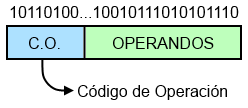
\includegraphics{res/tema1/instrucciones.png}
\end{center}

En la arquitectura de un computador Von Neumann, se tiene un modelo de computación que está basado en 3 conceptos básicos:
\begin{itemize}
\item Los datos y las instrucciones del programa a ejecutar están almacenadas en una \emph{única} memoria de lectura/escritura que denominamos la \emph{memoria principal}. Se denomina modelo de programa almacenado.
\item La memoria principal del computador Von Newmann es accesible por direcciones, lo que significa que cada uno de los contenidos de memoria es accesible sólo con su dirección.
\item La ejecución de las instrucciones en un computador Von Newmann es secuencial, es decir, una instrucción tras otra.
\end{itemize}

\section{Unidades principales}
\begin{center}
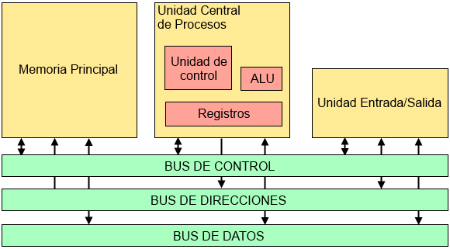
\includegraphics{res/tema1/unidadesppales.png}
\end{center}
\begin{itemize}
\item \emph{Memoria Principal}--- Contiene las instrucciones y los datos.
\item \emph{Unidad de Entrada y Salida}--- Conecta el procesador con el resto de periféricos.
\item \emph{Unidad Central de Procesos}--- Ejecuta las instrucciones. Esta formado a su vez por 3 unidades básicas:
\begin{enumerate}
\item Unidad Aritmético Lógica--- Realiza las operaciones aritmético-lógicas de las instrucciones.
\item Unidad de Control--- Controla el computador. Da las ordenes para que los elementos del computador trabajen correctamente. Estas han de recibirse en momentos precisos dependiendo del estado del procesador, por lo que esta conectado a todos los elementos del procesador. Las instrucciones que manda son denominadas Instrucciones de Control.
\item Registros--- Elementos de almacenamiento temporal de datos de máxima velocidad de acceso.
\end{enumerate}
\end{itemize}
Conectando todos estos elementos, están los buses de datos. Conectan las diferentes partes del procesador, y la salida hacia el resto del sistema.
\\
Existen 3 tipos de buses:
\begin{itemize}
\item \emph{Bus de Direcciones}--- Direcciona la memoria principal según lo que ordene el procesador.
\item \emph{Bus de Datos}--- Vuelca los datos entre la memoria y el procesador
\item \emph{Bus de Control}--- Manda las instrucciones (señales) del procesador para controlar otros elementos.
\end{itemize}

\section{La memoria principal}
\subsection{Direccionamiento}
Está compuesta por un conjunto de celdas del mismo numero de bits, donde se almacenan los datos y las instrucciones (Característica del modelo Von Neumann). 
A estas celdas se las denomina \emph{palabra de memoria}. 
Cada una de estas tiene asignada una dirección (0...2$^{n-1}$).
Para acceder a las palabras de memoria, basta con dar la dirección de la misma. Este sistema se denomina \emph{direccionamiento a palabra}.
\begin{center}
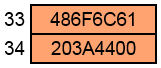
\includegraphics{res/tema1/memoriapalabra.png}
\end{center}
Existe otra forma de direccionar, que consiste en direccionar en vez de a palabra, a byte. Por ejemplo, en un sistema con una memoria de 32 bits de tamaño de palabra, una de estas contiene 4 bytes. En este sistema, cada uno de estos bytes tiene una dirección. Se denomina  \emph{direccionamiento a byte}.

\begin{center}
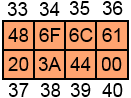
\includegraphics{res/tema1/memoriabyte.png}
\end{center}

Si el direccionamiento es a palabra, aumentamos de 1 en 1 la dirección para acceder a la siguiente palabra, y si el direccionamiento es a byte, hay que sumar el numero de bytes que puede almacenar una palabra si queremos acceder a la \textquotedblleft celda de abajo\textquotedblright
\subsection{Operación}
Para acceder a la memoria, necesitamos usar los 3 buses del procesador. La unidad de control, primero coloca en el bus de direcciones \emph{(el cual necesita n bits para poder acceder a  todas las direcciones de memoria)}, la dirección a la que quiere acceder. Entonces se manda por el bus de control la orden de acceso a memoria \emph{(memory request (MR))}, acompañada del flag del tipo de acceso que se está realizando (lectura o escritura \emph{[R/W]}).

Si se trata de un acceso de lectura, el contenido de esa dirección se recogerá entonces en el bus de datos, una vez transcurrido el tiempo de acceso que especifique el tipo de memoria.

Si se trata de un acceso de escritura, el procesador también ha de colocar en el bus de datos la información que se quiere grabar en esa dirección, y podrá quitar del bus la información una vez transcurrido el tiempo de escritura que especifique el tipo de memoria.

Es importante destacar que la escritura es destructiva, mientras que la lectura no lo es.
\subsection{Organización}
La información está habitualmente ordenada. En una zona está el código (las instrucciones), después hay una zona para los datos (estáticos o dinámicos). Al final de la memoria se sitúa la pila. Es una zona de almacenamiento que permite almacenar información y sacarla después, con un tipo de cola LIFO \emph{(Last In, First Out)}.
\\\\
La memoria tiene 3 características principales que la definen:
\begin{enumerate}
\item \emph{Capacidad}--- Se determina como el número de direcciones por el número de bits de cada dirección. También puede describirse en bytes. (Y normalmente este es el caso). Los tamaños típicos rondan los 256Mb a 16Gb en adelante.
\item \emph{Tiempo de acceso}--- Determinan los tiempos de lectura/escritura de la memoria. Normalmente están entre los 60$\sim$100 ns.
\item \emph{Tamaño de palabra}
\end{enumerate}
\section{Unidad Central de Proceso}
\subsection{Unidad Aritmético Lógica}
El ALU realiza las operaciones lógicas y aritméticas sobre cadenas de bits de longitud fija. Tiene 2 operandos, y se trata de un circuito digital, por lo que tiene señales de control que le permiten seleccionar la operación. Sólo puede ejecutar las ordenes para la que está diseñado. Los operandos pueden estar sobre registros o sobre memoria.
La ALU tiene un registro especial asociado, el \emph{registro de estado (RE)}. Este registro opera usando los diferentes bits del mismo como flags, y contienen información sobre la \emph{última} operación que se llevó a cabo en la ALU. Cada vez que la ALU realiza una operación, se actualiza el registro para reflejar el resultado de la misma. Los flags mas importantes son:
\begin{itemize}
\item Z \textrightarrow Resultado Cero (Se pone a valor 1 el flag si el resultado aritmético ha sido exactamente cero)
\item OVF \textrightarrow Overflow
\item C \textrightarrow Acarreo (Carry)
\item Paridad, etc...
\end{itemize}
La salida del RE sirve para toma de decisiones, principalmente saltos condicionales.
\subsection{Modelo de ejecución del computador}
El modelo de ejecución de un computador viene definido por el lugar donde se encuentran los operandos en una instrucción aritmético-lógica. Hay 3 posibles modelos:
\begin{itemize}
\item Registro a registro (los 2 operandos en el registro)
\item Registro a memoria (un operando en registro, y otro en memoria)
\item Memoria a memoria (los 2 operandos en memoria)
\end{itemize}
Cada modelo de ejecución contiene al anterior. P.E; en el modelo de memoria a memoria pueden provenir también de registros.
\subsection{Registros}
Son elementos de almacenamiento temporal, ubicados en el procesador. Son extremadamente rápidos. Hay de 3 tipos:
\begin{itemize}
\item de propósito general
\subitem Banco de registros
\item de propósito específico
\subitem PC \textrightarrow Contador de Programa (Program Counter)
\subitem SR \textrightarrow Registro de Estado (State Regisry)
\subitem SP \textrightarrow Puntero de Pila (Stack Pointer)
\item transparentes
\subitem IR \textrightarrow Registro de Instrucción (Instruction Register)
\subitem AR \textrightarrow Registro de Direcciones (Adress Register)
\subitem IR \textrightarrow Registro de Datos (Data Register)
\end{itemize}
Los registros de propósito general se usan explícitamente en el juego de instrucciones del computador. Pueden ser usados por cualquier instrucción que lleve a cabo operaciones sobre datos. Se suelen agrupar en bancos de registros, y tienen un tamaño igual al de la palabra.

Los registros de propósito específico tienen su uso restringido a determinadas instrucciones, y suelen usarlo de forma implícita.

Los registros transparentes son los que usa internamente el procesador, y no se especifican en las instrucciones. No son accesibles fuera de la unidad central de proceso.

Dos de los registros invisibles se usan para acceder a la memoria. Cada vez que hay que direccionar, la CPU carga la dirección en el Registro de Direcciones(AR), y manda la señal de control de READ y MEMORY ENABLE. Los datos de esa dirección se cargan tras el tiempo de acceso en el Registro de Datos (DR). En la escritura, se carga el dato en el DR, y la dirección de memoria en el AR, y se lanzan las señales de ME, y WRITE. El DR por ende se puede cargar de 2 sitios, desde la memoria o desde el procesador.

\subsection {Unidad de Control}
Es el tercer elemento que forma parte de la CPU. Es la encargada de leer las instrucciones de la memoria, de decodificarlas, analizarlas, y dar las ordenes a todos los elementos del procesador para su ejecución. Se trata de un circuito digital muy complejo, ya que han de funcionar todas las señales en momentos específicos. Se trata de un circuito síncrono, controlado por los pulsos generados por el reloj de la CPU (CLK). Este reloj indicará la velocidad a la que se realizan las operaciones en el procesador.

El procesador lee el registro de instrucción (IR) y el registro de estado (SR), y toma decisiones basado en estos. En cada ciclo/periodo de reloj, genera las señales de control asociadas a ese momento específico de ejecución, señales para la ALU, señales para el banco de registros, acceso a los buses, etc...

Es importante tener en cuenta que no todas las instrucciones se ejecutan en el proceso de un ciclo de CPU, y que los elementos más lentos de esta son la memoria y la ALU.

\subsection{Fases de ejecución de una instrucción}
\emph{Es importante no confundir la fase de ejecución con la ejecución en global.}
La ejecución de una instrucción se divide en 3 partes:

\begin{itemize}
\item Fase de fetch
\subitem Leer la instrucción de la memoria, de la dirección del PC.
\subitem Cargar la instrucción en el Registro de Instrucciones (IR)
\subitem Incrementar el PC para que apunte a la siguiente palabra.
\item Decodificación
\item Fase de Ejecución
\subitem Búsqueda de operandos.
\subitem Operación
\subitem Almacenamiento de Resultado.
\end{itemize}

La fase de fetch (o fase de búsqueda) es igual para todas las instrucciones. Todas tienen fase de fetch, y en todas tarda lo mismo. En esta fase, se lee la instrucción de la memoria principal de la dirección almacenada en el PC; se carga esta en el Registro de Instrucción (RI), y se incrementa el valor del PC para que este contenga ahora la dirección de la siguiente palabra. Los ciclos que tarde toda esta operación dependerá del procesador, la memoria...

A la decodificación le asignamos un ciclo de reloj.

La fase de ejecución, como máximo, lo que hará será: buscar los operandos; ya bien se encuentren en registro o en memoria, realizar la operación en sí, y almacenar el resultado de esta. Hay instrucciones que no tienen fase de ejecución, como los saltos condicionales; como por ejemplo, si no se cumple la condición de salto.
\\\\
Observemos un ejemplo de ejecución:
\begin{verbatim}
sub .r1,.r1,.r2
\end{verbatim}
R1 \textleftarrow R1 + R2
\begin{itemize}
\item Fase de fetch: 
\subitem Se lleva al AR el contenido del PC, y se realiza el acceso READ a la memoria principal. 
\subitem Se carga en el DR la instrucción que estaba contenida en la memoria.
\subitem Se lleva la instrucción del DR al IR.
\subitem Se incrementa el PC en 1 palabra.
\item Decodificación
\item Fase de Ejecución:
\subitem Se cargan r1 y r2 del banco de registros a la ALU, y se le indica el tipo de operación.
\subitem Se realiza la operación y se actualiza SR.
\subitem Se guarda el resultado en R1.
\end{itemize}

En un juego de instrucciones de un compilador hay diferentes tipos de instrucciones. Hay instrucciones que puede ejecutar el usuario, y otras que solo las puede ejecutar el sistema operativo. El usuario solo dispone de un subconjunto de las operaciones, que puede ejecutar en modo usuario. El S.O. es el que puede ejecutar las ordenes privilegiadas.

\section{Unidad de Entrada/Salida}
Es la encargada de realizar la conexión y el intercambio de información entre la CPU y los periféricos. Es necesaria porque los periféricos y el procesador tienen características muy diferentes, y difieren mucho en velocidad y tamaño de información que manejan. Esta unidad está compuesta por módulos de E/S que ocultan las particularidades de cada periférico. Además, es la encargada de la comunicación con el computador. Los módulos a su vez están constituidos por varios registros, que son en general el de datos, el de control y el de estado.

Hay 2 problemas básicos a resolver para que los periféricos se comuniquen con la CPU.
\subsection{Direccionamiento de los dispositivos}

Se refiere a cómo seleccionar el periférico con el que se establecerá la comunicación. Se hace asignando a cada registro del modulo de E/S una dirección. Se selecciona a través del bus de direcciones. Con respecto a esta asignación de direcciones de módulos E/S, existen a su vez otras 2 posibilidades:
\begin{itemize}
\item \emph{Mapa de E/S y Memoria Principal Común} Parte de la memoria principal se usa para E/S, y dichas direcciones están protegidas. No se pueden usar las mismas direcciones para E/S y memoria principal. Esto implica que no es necesario usar señales de control diferentes ni instrucciones diferentes. Como el mapa de instrucciones es común, adicionalmente se pueden usar instrucciones de carga y almacenamiento en memoria sobre dichas direcciones.
\item \emph{Mapa E/S y Memoria Principal Separados} Al ser 2 mapas diferentes, se pueden usar direcciones correlativas, ya que se especifica si se accede a la memoria principal o a la modulo de E/S. Por ejemplo, \emph{MemQR(1000)} y \emph{IOQR(1000)} tendrán como resultado el contenido de la memoria principal en la dirección 1000, o el contenido de memoria de I/O [E/S en inglés, Input/Output] en la dirección 1000. Adicionalmente, se dispondrán de instrucciones específicas para la E/S.
\end{itemize}
\subsection{Modos de realizar la transferencia E/S}
La operación de transferencia de E/S se puede establecer de 3 modos:
\begin{itemize}
\item \emph{E/S Programada} En este modo, es la CPU la que se encarga de controlar todo el proceso de E/S. Esto quiere decir, que comprueba el estado del periférico y si está preparado para comunicarse, envía o recibe el dato y continua la CPU con la siguiente instrucción. A ciclos regulares comprueba dichos estados. La CPU tiene entonces que estar observando el estado de los periféricos, esto es inconveniente ya que se pierde tiempo de procesador en realizar estas operaciones, y por ende, disminuye la productividad de la máquina.
\item \emph{E/S por interrupciones} En este modo, es el periférico el que a través del módulo de E/S avisa a la CPU de que está preparado para la transferencia, y lo hace mediante una señal, denominada \emph{Señal de interrupción}. Cuando observa la CPU la señal de interrupción, el procesador hace la transferencia. Se ahorra tiempo, pero se sigue gastando tiempo en comprobar dicha señal. Al recibir la interrupción, la CPU interrumpe la ejecución del programa, salva el estado de la máquina y ejecuta un miniprograma denominado \emph{rutina de tratamiento de la información}. Esta da servicio al periférico que ha interrumpido. Es una rutina que se ejecuta en modo privilegiado. Una vez que ha terminado de dar servicio, restaura el estado del programa, y continúa con la ejecución del mismo. La CPU comprueba si hay interrupción \emph{después} de ejecutar cada instrucción. Las interrupciones se tratan como saltos condicionales, son bifurcaciones condicionales por una condición externa. La ventaja de este modo es que el tiempo ocupado por el procesador en las operaciones de E/S es mucho menor que en la E/S programada.
\item \emph{Acceso Directo a Memoria (DMA)} En el DMA, la CPU sólo inicia la operación de E/S, es decir, ordena la transferencia pero no ejecuta instrucciones para producirla, con lo que puede ejecutar otras instrucciones mientras. Es el módulo de E/S el que accede directamente a memoria. Cuando el módulo acaba, envía otra señal para indicarlo. El problema de esto es que como se comparten los buses, estos pueden estar ocupados. Hay que implementar mecanismos para la gestión de buses. Pueden usarse memorias multipuerto, robo de ciclo, o otras tecnologías.
\end{itemize}

\section{Diseño de programas}
En un computador Von Neumann, para que se puedan ejecutar programas, las instrucciones y los datos han de estar en el mismo lugar. Existen herramientas de diseño que nos ayudan a crear programas.
\begin{itemize}
\item \emph{Compilador} Genera a partir de un lenguaje de alto nivel un programa en lenguaje máquina (el programa objeto). Es el ejecutable, y puede ejecutarse tantas veces como se desee.
\item \emph{Programa Ensamblador} El código máquina viene derivado de un lenguaje máquina, también denominado Ensamblador (Assembler, asm), que lo genera dentro del compilador un programa ensamblador. Todavía las ordenes no están en binario, pero tienen una correlación directa con el. El ensamblador transforma dicho lenguaje máquina en el código máquina. Cada programa ensamblador viene derivado del juego de instrucciones del procesador para el cual está diseñado.
\item \emph{Cargador} Es el encargado de transferir a memoria principal el programa desde el almacenamiento secundario.
\item \emph{Sistema Operativo} Realiza la gestión de los recursos de la máquina, y tiene otras funciones, como ocultar la complejidad de los periféricos y la protección de los recursos (para que el usuario no pueda realizar operaciones invalidas o maliciosas. El núcleo del sistema operativo se ejecuta en modo privilegiado.
\end{itemize}

\section{Parámetros Característicos}
\begin{itemize}
\item \emph{Ancho de Palabra} Es el número de bits que maneja en paralelo el procesador. En general, coincide con el tamaño de los registros y del bus de datos.
\item \emph{Tamaño de Memoria} Se expresa en bytes.
\item \emph{Frecuencia de Reloj} Determina la velocidad a la que se realizan eventos en la máquina. La inversa de este es el ciclo.
\item \emph{Capacidad de Cómputo} Tambien denominado productividad, velocidad, o throughput. Es el trabajo útil partido del tiempo. Se puede medir en MIPS, Millions of Instructions per Second (Millones de instrucciones por cada segundo), y en MFLOPS, Million of Floating Operations per Second (Millones de operaciones de coma flotante por cada segundo).
\item \emph{Ancho de Banda} Cantidad de información que es capaz de transmitir una unidad del computador.
\end{itemize}

\chapter{Ensamblador}
\section{Lenguaje Máquina}

El lenguaje máquina está formado por datos e instrucciones almacenados en memoria en forma binaria; específico para cada computador. El programa está constituido por instrucciones, que son las unidades elementales auto-contenidas que ejecuta el computador. Realizan una única y sencilla orden, y tienen un número fijo de operandos.

En general se ajustan a la palabra del computador, pero también se pueden tener instrucciones de 2 y media palabra. El juego de instrucciones son las posibles instrucciones que ejecuta el computador.
 
El formato de la instrucción es la representación de cada campo. El juego de instrucciones tiene el número de formas mas básico posible. Los operandos son la ubicación, que muchas veces nombramos como dirección, de los operandos. Estos pueden estar en la propia instrucción, en los registros, o en la memoria. Dependiendo de donde esté, se especifica como veremos más adelante. El campo de operandos puede estar dividido en suboperandos. Cuando los operandos son implícitos, puede no tener operandos la instrucción.

Se plantean 4 posibilidades para la separación en suboperandos:
\begin{itemize}
\item \emph{0 Direcciones} \textrightarrow Cuando los operandos son implícitos.
\item \emph{1 Dirección} \textrightarrow En general, la dirección es el origen y el destino.
\item \emph{2 Direcciones} \textrightarrow En general, el primero es origen y destino, y el operando 2 origen.
\item \emph{3 Direcciones} \textrightarrow El operador 1 origen, y los operadores 2 y 3 destinos.
\end{itemize}

\subsection{Tipos de datos}
\begin{itemize}
\item Palabras(tamaño privilegiado del procesador), medias palabras, bytes.
\item Acceso a memoria 
\subitem A palabra \textrightarrow Cada palabra tiene una dirección.
\subitem A byte \textrightarrow Cada byte tiene una dirección.
\item Alineación a palabra \textrightarrow Se direcciona al primer byte de la palabra.
\item Ordenación de bytes en memoria
(TODO AGREGAR DIBUJOS)
\subitem \emph{Little Endian} Al LSB (Least Significant Bit, Bit menos significativo) le corresponde la dirección menor.
\subitem \emph{Big Endian} Al MSB (Most Significant Bit, Bit mas significativo) le corresponde la dirección menor.
\end{itemize}

\subsection{Lenguaje Ensamblador (IEEE 694)}
La traducción ensamblador/código máquina es inmediata. En lenguaje ensamblador, las instrucciones vienen definidas por un código nemónico y unos nombres simbólicos mientras que las instrucciones en código máquina son códigos binarios. (P.E. load \textrightarrow \verb|ld|)

Las instrucciones en asm tienen la misma organización y estructura que las instrucciones máquina.

(TODO AGREGAR DIBUJO INSTRUCCION - asm)

Los nombres simbólicos que se utilizan para nombrar a las instrucciones son verbos de acción y códigos nemónicos de dichos verbos.
\begin{quote}
add \textrightarrow \verb|add|	load \textrightarrow \verb|ld|
branch \textrightarrow \verb|br|	store \textrightarrow \verb|st|
\end{quote}
 
\section{Modos de Direccionamiento}
\begin{itemize}
\item \emph{Inmediato} \verb|#valor| \textrightarrow En binario o en complemento a 2.
\item \emph{Directo} 
	\begin{itemize}
	\item Absoluto
		\begin{itemize}
		\item \emph{Registro} \verb|.registro|
		\item \emph{Memoria} \verb|/dirMemoria|
		\end{itemize}
	\item Relativo
		\begin{itemize}
		\item \emph{Registro Base} \verb|#desp[.registro]|
		\item \emph{Registro Indice} \verb|#desp[.registroIndice]|
		\item \emph{PC} \verb|$desp|
		\end{itemize}
	\end{itemize}
\item \emph{Indirecto}
	\begin{itemize}
	\item \emph{Registro} \verb|[.registro]|
	\item \emph{Memoria} \verb|[/dirMemoria]|
	\end{itemize}
\item \emph{Implícito}
\end{itemize}
\subsection{Direccionamiento Inmediato}
En el direccionamiento Inmediato, el objeto está contenido dentro de la propia instrucción. Son valores directos. \verb|ADD .R1,#4| En este caso, \verb|#4| es el valor que se sumará a R1.  \emph{R1 \textleftarrow R1+4}.
\subsection{Direccionamiento Directo}
En este direccionamiento, el objeto no está en la instrucción, esta contiene la información de donde está. Hay dos tipos de direccionamientos inmediatos, los absolutos, los cuales contienen la dirección completa, y los relativos, los cuales todos se refieren a la memoria principal, y tienen suficiente información para calcular cual es la dirección del objeto.
\subsubsection{Direccionamiento Directo Absoluto a Registro}
También denominado Direccionamiento Directo a Registro. En este direccionamiento, el objeto se encuentra en un registro. Lo que contienen la instrucción es la especificación de cual registro es.
\subsubsection{Direccionamiento Directo Absoluto a Memoria}
También denominado Direccionamiento Directo a Memoria. El objeto se encuentra en una dirección de memoria. La instrucción contiene la dirección completa de memoria.
\subsection{Direccionamientos Relativos}
En este tipo de direccionamientos el objeto está contenido en una dirección de memoria, pero la instrucción no contiene la dirección absoluta, sino información para calcularla.
\subsubsection{Direccionamiento Relativo a Registro Base}
El registro base contiene una dirección de memoria. Para calcular la dirección de memoria del objeto, se le suma un desplazamiento a la dirección contenida en el registro. Luego, la dirección del objeto es la dirección contenida en el registro base, mas el desplazamiento. El contenido del registro base no se altera, el desplazamiento no se aplica de forma destructiva.
\subsubsection{Direccionamiento Relativo a Program Counter (PC)}
En estas ordenes el PC está implícito. El PC es el registro base. Lo único que se especifica en este direccionamiento es el valor del desplazamiento. Estas cargan en el PC otra dirección. Esto nos permite hacer saltos cercanos. Según el estándar IEEE694, el PC se incrementa en el fetch, luego se aplica el desplazamiento sobre PC+1 palabra. (En el M88110 se verá que esto no es así para ese procesador). Es desplazamiento se carga con signo.
\subsubsection{Direccionamiento Relativo a Registro Índice}
Este desplazamiento tiene un registro base, pero en este desplazamiento se altera el contenido del registro base. La dirección del objeto, al igual que con el desplazamiento relativo a registro base, se calcula sumando la dirección del registro, y la del desplazamiento, pero con una modificación.
El contenido de este registro se modifica con un pre/post incremento/decremento.
\begin{itemize}
\item \emph{Preincremento}: Se incrementa el valor del registro \emph{antes} de calcular la dirección.
\item \emph{Predecremento}: Se decrementa el valor del registro \emph{antes} de calcular la dirección.
\item \emph{Postincremento}: Se incrementa el valor del registro \emph{después} de calcular la dirección.
\item \emph{Postincremento}: Se decrementa el valor del registro \emph{después} de calcular la dirección.
\end{itemize}
El tamaño del incremento/decremento es igual al tamaño del objeto transferido (palabra).
\subsection{Direccionamiento Indirecto}
En IEEE 694 se permiten todas las posibilidades, aquí solo vamos a ver algunas. La instrucción contiene la dirección del objeto. Pueden existir varios niveles de indirección. Hay 2 formas de realizar direccionamientos indirectos, a registro y a memoria.
\subsubsection{Direccionamiento Indirecto a Registro}
La instrucción contiene la especificación del registro, el cual contiene la dirección del objeto. Cuando solo hay un nivel de indirección es parecido al registro base con desplazamiento 0. Cuando hay varios niveles de indirección, el registro contiene la dirección de memoria que contiene la dirección de memoria del objeto. \verb|[[.R1]]| \textrightarrow 2 corchetes.
Puede contener desplazamientos. Adicionalmente, permite pre/postincrementos y pre/postdecrementos.
\subsubsection{Direccionamiento Indirecto a Memoria}
La instrucción contiene una dirección de memoria, la cual contiene la dirección del objeto. \verb|LD .R1,[/1000]| es R1 \textleftarrow MEM(MEM(1000)).
\subsection{Direccionamiento Implícito}
En la instrucción no hay información ni sobre la dirección ni sobre el objeto. Para los operandos no implícitos de la instrucción, son posibles todos los direccionamientos que hemos visto. En una instrucción, pueden coexistir modos de direccionamiento diferentes.
\subsubsection{Direccionamiento Implícito a Pila}
Es un tipo de direccionamiento en el que el puntero de pila (SP) es implícito. El SP puede apuntar a la primera posición libre o ocupada de la pila. A su vez, la pila puede crecer hacia direcciones de memoria crecientes o decrecientes.
Aunque el sistema no tenga una pila gestionada por el procesador, se puede hacer una pila a mano, seleccionando una zona en memoria que será usada para la pila, y usando como SP un registro de propósito general.
Supongamos que la pila está implementada en memoria. Hay 2 instrucciones que trabajan con la pila, \verb|PUSH| y \verb|POP|. \verb|PUSH| es guardar en la pila, \verb|POP| es sacar de la pila. El procesador automáticamente actualiza SP y gestiona la pila.
\verb|TODO: ¿METO AQUI LOS EJEMPLOS DE OPERACION DE LA PILA?|
\section{Juego de Instrucciones}
El juego de instrucciones es el conjunto de las instrucciones de un computador especifico. Son las herramientas con las que se construye un programa. Hay muchos tipos de tipos de instrucciones.
\subsection{Transferencia de Datos}
Mueven los datos entre registros y memoria. No modifican los biestables de estado. Copian el origen en el destino, sin modificar el origen.
\begin{itemize}
\item \verb|LD| (load) Cargar un registro. [DEST(REG), ORIG(INMM/DIR.MEM.)]
\item \verb|ST| (store) Almacenar en memoria. [ORIG(INMM/REG), DEST(DIR.MEM)]
\item \verb|MOVE| (move) Mueve un objeto. [ORIG, DEST]  REG a REG ó MEM a MEM
\end{itemize}
\subsection{Bifurcaciones (o Saltos)}
Modifican la estructura de flujo del programa. Cargan el PC con la dirección de la bifurcación (la siguiente instrucción que se ejecutará). No modifican el SR
\subsubsection{Incondicionales} 
\verb|BR| (branch). Siempre que se ejecuta, salta a la dirección de la instrucción. No hay una condición para el salto. Detrás de la instrucción \verb|BR|, tiene que haber una dirección de memoria, indicada por cualquier modo de direccionamiento.
\subsubsection{Condicionales}
También tienen que tener una dirección con los diferentes modos de direccionamiento. Saltan si se cumple la condición de salto (que coincida el estado del bit de estado con el estado esperado). Si no coincide no hace nada.
Saltos comunes
\begin{itemize}
\item \emph{Z} \textrightarrow Zero
\item \emph{NZ} \textrightarrow Not Zero
\item \emph{C} \textrightarrow Carry (Accareo)
\item \emph{NC} \textrightarrow No Carry (Sin acarreo)
\item \emph{V} \textrightarrow Overflow (Desbordamiento)
\item \emph{NV} \textrightarrow No Overflow (Sin Desbordamiento)
\item \emph{P} \textrightarrow Par
\item \emph{N} \textrightarrow Negativo
\end{itemize}
Usan los estados de la última operación de la ALU.
\subsubsection{Con Retorno}
Se utilizan para implementar subrutinas (macros). En estas, se salta y se vuelve mas adelante, al contrario de los otros saltos.
Una subrutina es un segmento de código, al que se pueden saltar desde otros programas. Se accede a las subrutinas con \verb|CALL|, (llamada a subrutina). En las subrutinas, hay un comando para salir de la misma, \verb|RET|. Esta instrucción es implícita, y continua con la ejecución del programa después del \verb|CALL|.
\verb|CALL| guarda el PC, y \verb|RET| lo recupera. Existen 2 sitios para guardar el PC
\begin{itemize}
\item Un registro de carácter general, con lo que no se permiten llamadas anidadas, ya que si no perderíamos las llamadas anteriores
\item En la pila, lo que permite llamadas anidadas, ya que podemos guardar todos los retornos que necesitemos. Hay que tener cuidado con la gestión de la pila para saber que estamos apuntando a la instrucción correcta.
\end{itemize}
\subsection{Aritméticas y Comparación}
IEEE permite 3 operandos y 4 operandos para la división.
[ORIG/DEST, ORIG] y [DEST, ORIG, ORIG]
\begin{itemize}
\item \verb|ADD| Suma \textrightarrow \verb|ADD .R1, .R2|
\item \verb|SUB| Resta \textrightarrow \verb|SUB .R1, .R2|
\item \verb|MUL| Multiplicación \textrightarrow \verb|MUL .R1, .R2|
\item \verb|DIV| División \textrightarrow \verb|DIV .R1, .R2|
\end{itemize}
\end{document}